\section{Decision Trees and Random Forests}

\subsection{Predictions from Decision Trees}

\mult{2}

\begin{definition}{Decision Tree}\\
A decision tree is a tree-like model of decisions where:
\begin{itemize}
    \item Each internal node represents a test on a feature
    \item Each branch represents an outcome of the test
    \item Each leaf node represents a prediction (class label or value)
\end{itemize}
Decision trees can be used for both classification and regression tasks.
\end{definition}

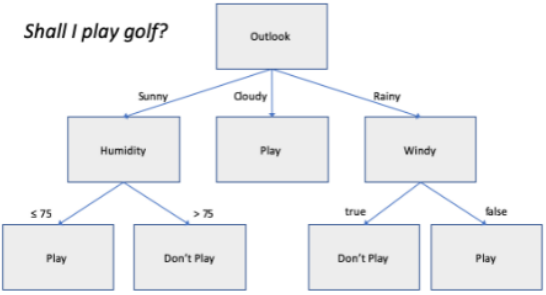
\includegraphics[width=0.8\linewidth]{decision_tree_example.png}

\multend

\mult{2}

\begin{formula}{Gini Impurity}\\
Gini impurity measures how often a randomly chosen element would be incorrectly labeled if labeled randomly according to the distribution of labels in the subset:
\[G(Q_i) = 1 - \sum_{k=1}^{K} p_{i,k}^2\]
where $p_{i,k}$ is the proportion of class $k$ observations in node $i$.
\end{formula}

\begin{definition}{Entropy}\\
Entropy is another measure of impurity:
\[H(Q_i) = -\sum_{k=1}^{K} p_{i,k} \log_2 p_{i,k}\]
Both Gini impurity and entropy are used in building decision trees.
\end{definition}



\begin{KR}{Making Predictions with Decision Trees}
\paragraph{For classification}
Follow the tree from root to leaf:
\begin{itemize}
    \item Start at the root node
    \item At each internal node, evaluate the feature test
    \item Follow the branch corresponding to the test outcome
    \item Continue until reaching a leaf node
    \item Return the majority class in the leaf as the prediction
\end{itemize}

\paragraph{For regression}
Follow the same process, but:
\begin{itemize}
    \item Return the average target value of training samples in the leaf
    \item Trees approximate the target function as a piecewise constant function
\end{itemize}

\paragraph{Prediction confidence}
For classification:
\begin{itemize}
    \item Confidence can be estimated from class proportions in the leaf
    \item For example, if a leaf has 80 samples of class A and 20 of class B:
    \begin{itemize}
        \item Predict class A with 80\% confidence
        \item Alternative: predict probabilities [0.8, 0.2]
    \end{itemize}
\end{itemize}
\end{KR}



\multend

\begin{example}{Decision Tree Classification}
Consider classifying iris flowers based on petal length and width:
\begin{itemize}
    \item Root node: ''Is petal length < 2.45 cm?''
    \item If yes: Predict Setosa (all samples with petal length < 2.45 cm are Setosa)
    \item If no: ''Is petal width < 1.75 cm?''
    \item If yes: Predict Versicolor
    \item If no: Predict Virginica
\end{itemize}
\end{example}

\begin{concept}{Node Purity and Splitting Criteria}\\
When building a decision tree, nodes are split to maximize ''purity'':
\begin{itemize}
    \item A pure node contains only samples of a single class
    \item Splits are chosen to maximize information gain
    \item Information gain is the reduction in impurity (Gini or entropy) after a split
    \item The cost of a split is the weighted average of child node impurities:
    \[J(Q_i, \theta) = \frac{m^{left}_i}{m_i}G(Q^{left}_i(\theta)) + \frac{m^{right}_i}{m_i}G(Q^{right}_i(\theta))\]
\end{itemize}
\end{concept}

\begin{example2}{Gini Impurity Calculation}
    $$
\begin{gathered}
T=1-\left(\frac{105}{144}\right)^2-\left(\frac{39}{144}\right)^2=0.395, \quad F=1-\left(\frac{34}{159}\right)^2-\left(\frac{125}{159}\right)^2=0.336 \\
\text { Tot }_{\text {Weighted }}=\left(\frac{144}{144+159} \cdot 0.395\right)+\left(\frac{159}{144+159} \cdot 0.336\right)=0.364
\end{gathered}
$$

\textbf{Gini coefficients:}
\begin{itemize}
    \item Chest Pain $=0.364$
    \item Good Blood Circulation $=0.360$
    \item Blocked Arteries $=0.381$
\end{itemize}
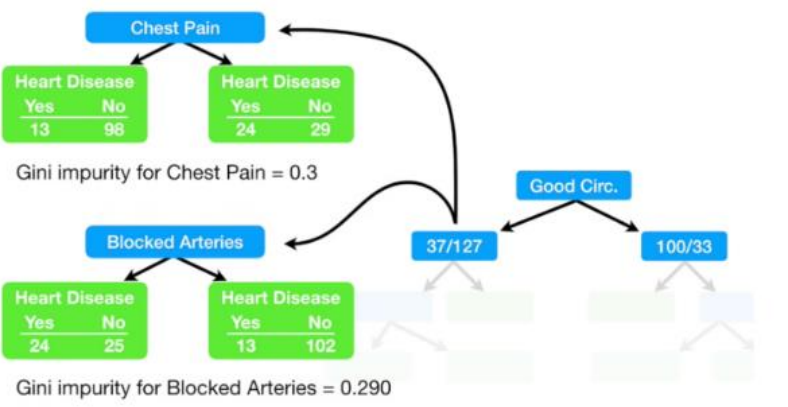
\includegraphics[width=0.8\linewidth]{gini_coefficients_example1.png}

\textbf{Step 2: Lowest Impurity = Root}
Root $=$ Good Blood Circulation

\textbf{Step 3: Calculate Gini Impurity for Branches}

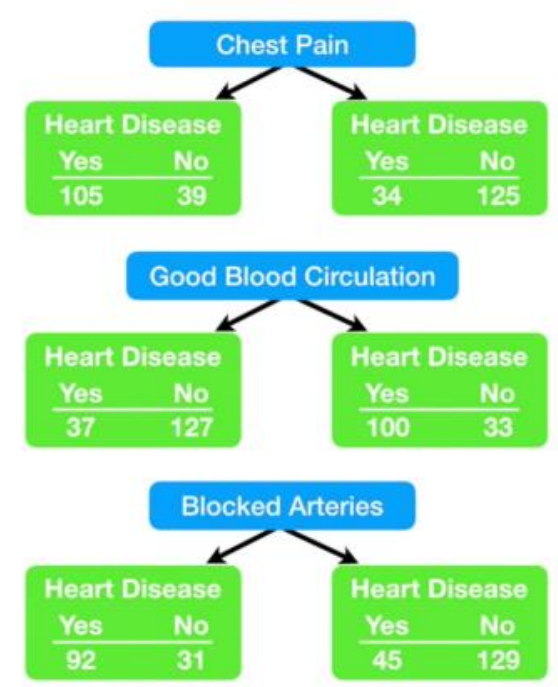
\includegraphics[width=0.5\linewidth]{gini_coefficients_example2.png}
    
\end{example2}


\subsection{Training Decision Trees}

\begin{KR}{Training a Decision Tree with CART Algorithm}
\paragraph{Start with root node}
Begin with all training samples in the root node

\paragraph{Find best split}
For each feature and potential threshold:
\begin{itemize}
    \item Calculate the cost function (e.g., Gini impurity or entropy for classification, MSE for regression)
    \item Choose the feature and threshold that minimizes the cost
\end{itemize}

\paragraph{Split the node}
Divide the data based on the best split found

\paragraph{Recursively build sub-trees}
For each child node, repeat steps 2-3 until stopping criteria are met:
\begin{itemize}
    \item Maximum depth reached
    \item Minimum samples per node threshold met
    \item Node becomes pure (all samples belong to same class)
\end{itemize}

\paragraph{Make predictions}
For classification: Predict the majority class in the leaf node
For regression: Predict the average value of samples in the leaf node
\end{KR}

\begin{concept}{Building Binary Trees}\\
The CART algorithm builds binary trees:
\begin{itemize}
    \item Each split creates exactly two child nodes (binary split)
    \item For categorical features with $p$ possible values, there are $2^{p-1} - 1$ possible binary partitions
    \item In practice, often use one-hot encoding for categorical features
\end{itemize}
\end{concept}

\begin{example2}{Training a Decision Tree}\\
Consider a dataset with two features (age and income) and a binary target (buy vs. don't buy):
\begin{itemize}
    \item 10 samples: 6 ''buy'' and 4 ''don't buy''
    \item Root node Gini impurity: $1 - (\frac{6}{10})^2 - (\frac{4}{10})^2 = 1 - 0.36 - 0.16 = 0.48$
\end{itemize}
\tcblower
Evaluate split on age = 30:
\begin{itemize}
    \item Left node (age < 30): 5 samples, 4 ''buy'' and 1 ''don't buy''
    \item Left node Gini: $1 - (\frac{4}{5})^2 - (\frac{1}{5})^2 = 1 - 0.64 - 0.04 = 0.32$
    \item Right node (age $\leq$ 30): 5 samples, 2 ''buy'' and 3 ''don't buy''
    \item Right node Gini: $1 - (\frac{2}{5})^2 - (\frac{3}{5})^2 = 1 - 0.16 - 0.36 = 0.48$
    \item Weighted Gini after split: $\frac{5}{10} \times 0.32 + \frac{5}{10} \times 0.48 = 0.16 + 0.24 = 0.40$
    \item Information gain: $0.48 - 0.40 = 0.08$
\end{itemize}

Evaluate split on income = 50K:
\begin{itemize}
    \item Left node (income < 50K): 6 samples, 2 ''buy'' and 4 ''don't buy''
    \item Left node Gini: $1 - (\frac{2}{6})^2 - (\frac{4}{6})^2 = 1 - 0.11 - 0.44 = 0.45$
    \item Right node (income $leq$ 50K): 4 samples, 4 ''buy'' and 0 ''don't buy''
    \item Right node Gini: $1 - (\frac{4}{4})^2 - (\frac{0}{4})^2 = 1 - 1 - 0 = 0$
    \item Weighted Gini after split: $\frac{6}{10} \times 0.45 + \frac{4}{10} \times 0 = 0.27 + 0 = 0.27$
    \item Information gain: $0.48 - 0.27 = 0.21$
\end{itemize}

The split on income = 50K has higher information gain, so it's selected for the root node.
\end{example2}

\raggedcolumns
\columnbreak

\subsection{Regularization in Decision Trees}

\begin{concept}{Regularization in Decision Trees}\\
Decision trees tend to overfit without regularization. Common regularization techniques include:
\begin{itemize}
    \item \textbf{Max depth}: Limit the maximum depth of the tree
    \item \textbf{Min samples split}: Require minimum number of samples to split a node
    \item \textbf{Min samples leaf}: Require minimum number of samples in leaf nodes
    \item \textbf{Max features}: Limit number of features considered for splitting
    \item \textbf{Pruning}: Remove branches that don't improve generalization
\end{itemize}
\end{concept}

\begin{KR}{Pruning Decision Trees}
\paragraph{Pre-pruning (early stopping)}
Stop growing the tree early by setting constraints:
\begin{itemize}
    \item Maximum depth
    \item Minimum samples required for splitting
    \item Minimum samples required in leaf nodes
    \item Minimum impurity decrease required for splitting
\end{itemize}

\paragraph{Post-pruning}
Grow a full tree, then prune back branches:
\begin{itemize}
    \item Grow a full, deep tree
    \item Evaluate performance on validation set
    \item Iteratively remove branches that don't improve validation performance
    \item Continue until pruning no longer improves performance
\end{itemize}

\paragraph{Cost-complexity pruning}
A systematic approach to post-pruning:
\begin{itemize}
    \item Define a cost-complexity measure that balances tree complexity and error
    \item Generate a sequence of trees with decreasing complexity
    \item Select the tree with best validation performance
\end{itemize}
\end{KR}

\begin{concept}{White Box vs. Black Box Models}\\
Decision trees are considered ''white box'' models because:
\begin{itemize}
    \item The decision-making process is transparent and interpretable
    \item You can see the exact rules and thresholds used for classification
    \item Each prediction can be explained by tracing the path through the tree
\end{itemize}
This contrasts with ''black box'' models like neural networks, where the decision-making process is opaque.
\end{concept}

\raggedcolumns
\columnbreak

\subsection{Random Forests}

\begin{definition}{Random Forest}\\
Random Forest is an ensemble learning method that combines multiple decision trees to improve prediction accuracy and control overfitting. Key aspects include:
\begin{itemize}
    \item Each tree is trained on a bootstrap sample of the training data (random sampling with replacement)
    \item When building trees, only a random subset of features is considered for splitting at each node
    \item Final prediction is made by averaging predictions (regression) or taking majority vote (classification) from all trees
\end{itemize}
\end{definition}

\begin{concept}{Bagging (Bootstrap Aggregating)}\\
Bagging is a technique to improve model stability and accuracy:
\begin{itemize}
    \item Generate multiple training sets by sampling with replacement from the original training data
    \item Train a separate model on each bootstrap sample
    \item Combine predictions by averaging (regression) or voting (classification)
    \item Reduces variance without increasing bias
\end{itemize}
\end{concept}

\begin{concept}{Out-of-Bag Evaluation}\\
In Random Forests, each tree is trained on a bootstrap sample, leaving some samples out (out-of-bag or OOB samples):
\begin{itemize}
    \item OOB samples act as a validation set for each tree
    \item For each sample, predictions are made only by trees that didn't use it for training
    \item OOB error provides an unbiased estimate of the generalization error
\end{itemize}
\end{concept}

\begin{KR}{Training a Random Forest}
\paragraph{Initialize the forest}
\begin{itemize}
    \item Define number of trees $n\_trees$
    \item Set parameters: max\_features, max\_depth, min\_samples\_leaf, etc.
\end{itemize}

\paragraph{Build individual trees}
For each tree:
\begin{itemize}
    \item Create bootstrap sample from training data
    \item Build decision tree considering only random subset of features at each split
\end{itemize}

\paragraph{Make predictions}
For a new data point:
\begin{itemize}
    \item Get prediction from each tree
    \item Aggregate predictions (average for regression, majority vote for classification)
\end{itemize}
\end{KR}

\begin{concept}{Feature Importance in Random Forests}\\
Random forests provide a natural way to measure feature importance:
\begin{itemize}
    \item For each feature, measure the increase in prediction error after permuting its values
    \item Features with large increases in error are more important
    \item Alternatively, measure the average decrease in impurity across all trees when a feature is used for splitting
\end{itemize}
This helps identify which features have the most predictive power.
\end{concept}

\begin{example}{Random Forest Application}
Consider a credit scoring application:
\begin{itemize}
    \item Task: Predict if a customer will default on a loan
    \item Features: Income, age, employment history, credit history, loan amount
    \item Model: Random forest with 100 trees
    \item Each tree uses a bootstrap sample (about 63\% of training data)
    \item At each node, only $\sqrt{5} \approx 2$ features are considered for splitting
    \item Results:
    \begin{itemize}
        \item Individual tree accuracy: 78-85\%
        \item Random forest accuracy: 92\%
        \item Feature importance: Credit history (40\%), income (25\%), loan amount (20\%), employment history (10\%), age (5\%)
    \end{itemize}
\end{itemize}
\end{example}

\begin{KR}{Tuning Random Forest Hyperparameters}
\paragraph{Number of trees (n\_estimators)}
\begin{itemize}
    \item Start with a large number (100-500)
    \item More trees generally improves performance but increases computation
    \item Performance often plateaus after a certain number
\end{itemize}

\paragraph{Maximum features (max\_features)}
\begin{itemize}
    \item For classification: Default is $\sqrt{n\_features}$
    \item For regression: Default is $n\_features/3$
    \item Try different values and use cross-validation
\end{itemize}

\paragraph{Tree constraints}
\begin{itemize}
    \item max\_depth: Controls maximum depth of trees
    \item min\_samples\_split: Minimum samples required to split
    \item min\_samples\_leaf: Minimum samples required in leaf nodes
\end{itemize}

\paragraph{Bootstrap options}
\begin{itemize}
    \item bootstrap: Whether to use bootstrap samples (True by default)
    \item max\_samples: Size of bootstrap samples
\end{itemize}
\end{KR}

\begin{concept}{Other Tree-Based Ensemble Methods}\\
Beyond random forests, other tree-based ensemble methods include:
\begin{itemize}
    \item \textbf{Extra Trees (Extremely Randomized Trees)}: Similar to random forests but uses random thresholds for splitting
    \item \textbf{Gradient Boosting}: Builds trees sequentially, each correcting errors of previous trees
    \item \textbf{AdaBoost (Adaptive Boosting)}: Focuses subsequent trees on examples previous trees misclassified
    \item \textbf{XGBoost, LightGBM, CatBoost}: Optimized implementations of gradient boosting
\end{itemize}
\end{concept}

